\icode{E-MI-MU-L3-261029-002}
如图所示，两根轻绳一端系于结点\(O\)，另一端分别系于固定环上的\(A\)、	\(B\)两点，\(O\)点下面悬挂一物体\(M\)，绳\(OA\)水平，拉力大小为\(F_1\)，绳\(OB\)与\(OA\)夹角\(\alpha =\)\,\qty{120}{\degree}，拉力大小为\(F_2\)。将两绳同时缓慢顺时针转过\qty{60}{\degree}并保持两绳之间的夹角\(\alpha\)始终不变，且物体始终保持静止状态。则在旋转过程中，下列说法正确的是\paren[]

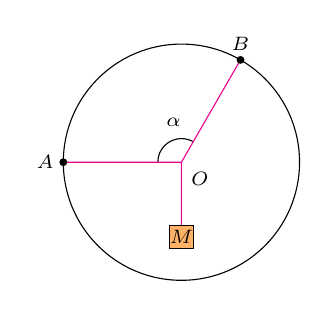
\begin{tikzpicture}[font=\scriptsize]
    \draw (0,0)node[below right]{\(O\)} circle(1.5) (-.3,0) arc(180:60:.3);
	\draw[magenta] (-1.5,0)--(0,0)--(60:1.5) (0,0)--(0,-.8);
	\draw[fill=orange!60] (-.15,-.8) rectangle(.15,-1.1)node[midway]{\(M\)};
	\fill (-1.5,0)node[left]{\(A\)} circle(.05) (60:1.5)node[above]{\(B\)} circle(.05);
	\node at(-.1,.5){\(\alpha\)};
\end{tikzpicture}
\begin{choices}
	\item\(F_1\)逐渐增大
	\item\(F_1\)先增大后减小
	\item\(F_2\)逐渐减小
	\item\(F_2\)先减小后增大
\end{choices}
\begin{answer}
    AC
\end{answer}